\begin{center}
	
	\begin{tabular}{rp{16cm}lp{20cm}}%{rl}
		
		% after \\: \hline or \cline{col1-col2} \cline{col3-col4} ...
		
		论文地址:& \href{https://dl.acm.org/doi/pdf/10.1145/3447548.3467237}{https://dl.acm.org/doi/pdf/10.1145/3447548.3467237} \\
		来源:& KDD, 2021 \\
		作者:& Shuanghong Shen, et al. \\
		单位:& USTC$_{\times 6}$, iFLYTEK Research\\
		源码:& \href{https://github.com/bigdata-ustc/EduKTM}{EduKTM} \\
		
		%  slides:& \href{http://yunshengb.com/wp-content/uploads/2017/03/nips_2018_r2l_workshop_talk.pdf}{{\footnotesize Convolutional Set Matching for Graph Similarity}}\\
		
		关键词:& \textbf{Knowledge Tracing, learning process, learning gain, forgetting effect} \\
		
		写于:& \date{2021-09-24}
		
	\end{tabular}
	
\end{center}

该论文\cite{shen2021learning}通过建模学生的学习过程来进行KT(Knowledge Tracing)。在以往的KT模型中,以高准确率为目标,认为高准确率代表准确的表示了学生的知识状态,这使得知识状态更多地与回答正确的练习相联系。除此之外,大部分DKT模型没有考虑learning gain(做完练习后对知识掌握水平的差别)和forgetting effect(学生的知识掌握水平会随着时间降低)。对此,论文提出了 Learning Processconsistent Knowledge Tracing (LPKT)。

\paragraph{问题定义}
形式化定义:练习集合$E = \{e_1, ..., e_J\}$,知识点集合$K = \{k_1, ..., k_M\}$,练习与知识点关系矩阵$Q \in \mathbb{R}^{J \times M}$表示每个练习包含了哪些知识点。

学生的学习过程表示为:$x = \{(e_1, at_1, a_1), it_1, (e_2, at_2, a_2), it_2, ..., (e_t, at_t, a_t), it_t\}$,其中$(e_i, at_i, a_i)$表示一个learning cell,分别表示练习、练习用时、回答,$it_i$表示相邻learning cell的时间间隔。LKPT将练习、回答、回答用时、时间间隔都转化为embedding。

LPKT的目标是给定学习序列,监控学生的知识状态以及预测学生回答下一个问题正确的可能性。

\paragraph{LPKT}
LPKT显示地建模了learning gain和forgetting effect。
\par{\textbf{learning gain}}\ \ \ \ LPKT将$t$时地learning cell转化为embedding $\boldsymbol{l}_t$,基于$\boldsymbol{l}_{t-1}, \boldsymbol{l}_t$和$it_t$的embedding得到$t$时的learning gain $\boldsymbol{lg}_t$,再将$\boldsymbol{lg}_t$通过learning gate(是一个向量,主要考虑的是学生吸收知识的能力)得到学生真实的learning gain。

\par{\textbf{forgettign effect}}\ \ \ \ LKPT设计了forgetting gate(一个向量,用于表示遗忘程度)。学生的知识状态的更新基于learning gain、学生上一时刻的知识状态和forgetting gate。

最终的预测基于学生更新后的知识状态和$e_{t+1}$的embedding计算得到。

LPKT模型结构如Fig.\ref{fig:lpkt}所示。
\begin{figure}[h]
	\centering
	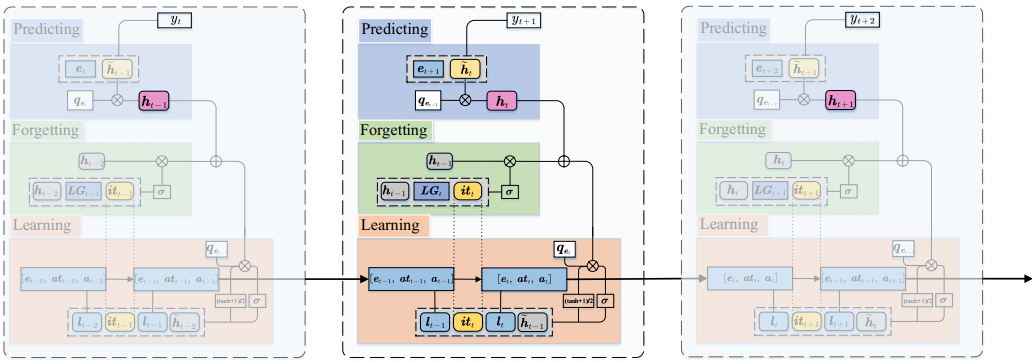
\includegraphics[width=\textwidth]{pics/lpkt.png}
	\caption{The architecture of the LPKT model}
	\label{fig:lpkt}
\end{figure}

论文使用的数据集:\href{https://sites.google.com/site/assistmentsdata/home/2012-13-school-data-withaffect}{ASSIST2012}、\href{https://sites.google.com/view/assistmentsdatamining/dataset}{ASSISTChall}、\href{http://ednet-leaderboard.s3-website-ap-northeast-1.amazonaws.com/}{EdNet-KT1},使用的指标有:RMSE、ACC、AUC、Pearson correlation。

\paragraph{总结}

\begin{itemize}
	\item LPKT考虑了learning gain和forgetting effect
	\item 将练习时间间隔加入到学习行为序列中
	\item 用矩阵表示学生的知识状态,每一行表示学生对一个知识点的掌握情况
	\item 只构建了练习与知识点之间的关系矩阵,\textbf{没有构建知识点之间的关系}
	
\end{itemize}

